\documentclass[notes]{beamer}
\usepackage{pgfpages}
\usetheme{Montpellier}
\usepackage{graphicx}
\usepackage{minted}

\title{Intro to Web Development \\ A Guided Tutorial}
\date{Updates as of: \today}

\begin{document}
\section{Introduction}
\begin{frame}
  \maketitle
\end{frame}

\begin{frame}{What we're covering}
  \begin{itemize}
    \item Review of HTML
    \item Basic JavaScript
    \item Examples of the Document Object Model (\textsc{dom})
    \item A hands-on example of building a todo-list page
  \end{itemize}
\end{frame}

\begin{frame}{What we'll be using}
    \begin{block}{Neocities}
    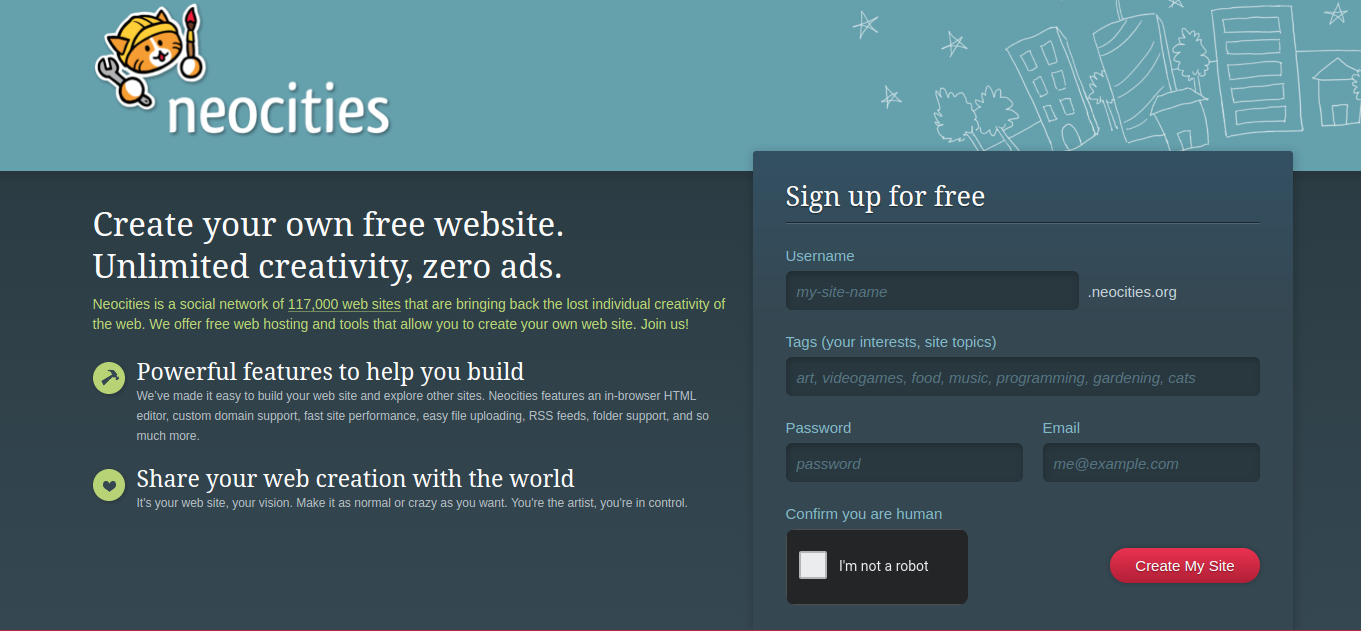
\includegraphics[width=4in]{../signup}
  \end{block}
\note{Neocities is a free hosting service that allows you to write all the code for your website. It's a pretty solid product that I highly recommend. There's a password provided for an in-class account that we'll be sharing, but if you want to continue working on your own you can sign up for your own account.}
\end{frame}


\begin{frame}{HTML \& JavaScript}
    \begin{block}{What are they}
    \begin{description}
      \item[HTML] \textbf Hyper\textbf Text \textbf Markup \textbf Language
      \item[JavaScript] A programming language
    \end{description}
  \end{block}
  \note{
    HTML is the like the bones, the architecture, of a webpage. It includes the basic \textit{content} of the webpage: there's a button here, a paragraph there, a link here. HTML by itself leads to very plain looking pages, like the ones we had in the 90s. You need CSS, which we aren't covering explicitly in this class, to make things look pretty.

    JavaScript is a \textit{programming language} that gives the web browser instructions on what to do in the web page. 
  }
\end{frame}

\begin{frame}{The DOM}
  \begin{block}{}
    {\Huge \textbf{D}ocument \textbf{O}bject \textbf{M}odel} 
  \end{block}
  \note{This is a technical term for ``the way that your JavaScript code can affect the web page''. The web page itself is the ``document'' and ``object'' references a kind of data inside the JavaScript language. By data we mean things like numbers or lists or pairs: information that the program needs to do its job. So the ``document object model'' means that the browser provides a way for your JavaScript code to understand the web page as data it can manipulate.}
\end{frame}

\begin{frame}{Our Example}
  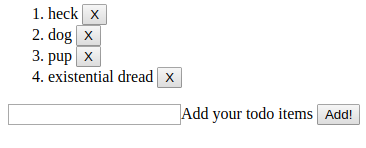
\includegraphics[width=3in]{FinalCodeScreenshot}
\end{frame}

\begin{frame}[fragile]{The first step}
  \begin{columns}
    \begin{column}{0.35\columnwidth}
      \begin{enumerate}
        \item On neocities, make a new file
        \item Call it ``YOURINITIALStodo.html''
        \item Type in exactly what you see on the right and save the file
        \item View the file
      \end{enumerate}
    \end{column}
    \begin{column}{0.65\columnwidth}
      \begin{minted}{html}
<html>
  
  <ol>
  </ol>

  <input>Add your todo items</input>
  <button>Add!</button>
</html>
    \end{minted}
    \end{column}
  \end{columns}
\end{frame}

\begin{frame}[fragile]{Your first touch of JavaScript}
  \begin{columns}
    \begin{column}{0.45\columnwidth}
      \begin{block}{Change your todo.html file}
        \begin{minted}[fontsize=\tiny]{html}
<html>
  <head>
    <script src="YOURINITIALStodo.js"></script>
  </head>
  <body>
    <ol>
    </ol>

    <input>Add your todo items</input>
    <button>Add!</button>
  </body>
</html>
        \end{minted}
      \end{block}
    \end{column}
    \begin{column}{0.45\columnwidth}
      \begin{block}{YOURINITIALStodo.js}
        \begin{minted}[fontsize=\tiny]{js}
window.onload = function () {
    console.log("Is this working?");
}          
        \end{minted}
      \end{block}
    \end{column}
  \end{columns}
\end{frame}

\begin{frame}[fragile]{Make the button do something}
  \begin{columns}
    \begin{column}{0.45\columnwidth}
      \begin{block}{Change your todo.html file}
        \begin{minted}[fontsize=\tiny]{html}
<html>
  <head>
    <script src="YOURINITIALStodo.js"></script>
  </head>
  <body>
    <ol id="list">
    </ol>

    <input id="input">Add your todo items</input>
    <button id="add">Add!</button>
  </body>
</html>
        \end{minted}
      \end{block}
    \end{column}
    \begin{column}{0.50\columnwidth}
      \begin{block}{Change your todo.js file}
        \begin{minted}[fontsize=\tiny]{js}
window.onload = function () {
    var inputElement = document.getElementById("input");
    var todoList = document.getElementById("list");
    var addButton = document.getElementById("add");

    addButton.addEventListener("click", function () {
      console.log("Is this working?");
    });
}        
        \end{minted}
      \end{block}
    \end{column}
  \end{columns}
\end{frame}

\begin{frame}[fragile]{Adding addition}

  \begin{block}{Change your todo.js file}
    \begin{minted}[fontsize=\tiny]{js}
window.onload = function () {
    var inputElement = document.getElementById("input");
    var todoList = document.getElementById("list");
    var addButton = document.getElementById("add");

    addButton.addEventListener("click", function () {
      console.log("Is this working?");
      var itemText = document.createTextNode(inputElement.value);
      var newItem  = document.createElement("li");
      newItem.appendChild(itemText);
      todoList.appendChild(newItem);
      inputElement.value = "";
    });
} 
    \end{minted}
  \end{block}
\end{frame}

\begin{frame}[fragile]{Delete buttons and <div>s}
  \begin{block}{Change your todo.js file}
    \begin{minted}[fontsize=\tiny]{js}
window.onload = function () {
    var inputElement = document.getElementById("input");
    var todoList = document.getElementById("list");
    var addButton = document.getElementById("add");

    addButton.addEventListener("click", function () {
      console.log("Is this working?");
      var itemText = document.createTextNode(inputElement.value + " ");
      var newItem  = document.createElement("li");
      var divvy = document.createElement("div");

      var deleteBut = document.createElement("button");
      var deleteText = document.createTextNode("X");

      deleteBut.appendChild(deleteText);
	
      divvy.appendChild(itemText);
      divvy.appendChild(deleteBut);
	
      newItem.appendChild(divvy);
      todoList.appendChild(newItem);
      inputElement.value = "";
    });
}    
    \end{minted}
  \end{block}
\end{frame}

\begin{frame}[fragile]{Adding IDs to the items}
  \begin{block}{Change your todo.js file}
    \begin{minted}[fontsize=\tiny]{js}
window.onload = function () {
    var inputElement = document.getElementById("input");
    var todoList = document.getElementById("list");
    var addButton = document.getElementById("add");

    var listIndex = 0;
    
    addButton.addEventListener("click", function () {
      console.log("Is this working?");
      var itemText = document.createTextNode(inputElement.value + " ");
      var newItem  = document.createElement("li");
      var divvy = document.createElement("div");
      var deleteBut = document.createElement("button");
      var deleteText = document.createTextNode("X");
      newItem.setAttribute("id","item"+listIndex);
      deleteBut.appendChild(deleteText);
      divvy.appendChild(itemText);
      divvy.appendChild(deleteBut);
      newItem.appendChild(divvy);
      todoList.appendChild(newItem);
      inputElement.value = "";
    });
}   
    \end{minted}
  \end{block}
\end{frame}

\begin{frame}[fragile]{Making the delete button work}
    \begin{minted}[fontsize=\tiny]{js}
window.onload = function () {
  var inputElement = document.getElementById("input");
  var todoList = document.getElementById("list");
  var addButton = document.getElementById("add");
  
  var listIndex = 0;
    
  addButton.addEventListener("click", function () {
    console.log("Is this working?");
    listIndex++
    var theIndex = listIndex;
    var itemText = document.createTextNode(inputElement.value + " ");
    var newItem  = document.createElement("li");
    var divvy = document.createElement("div");
    var deleteBut = document.createElement("button");
    var deleteText = document.createTextNode("X");
    newItem.setAttribute("id","item"+listIndex);
    deleteBut.appendChild(deleteText);
    deleteBut.addEventListener("click", function () {
      var theItem = document.getElementById("item"+theIndex);
      todoList.removeChild(theItem);
    });	
    divvy.appendChild(itemText);
    divvy.appendChild(deleteBut);	
    newItem.appendChild(divvy);
    todoList.appendChild(newItem);
    inputElement.value = "";
  });
}
    \end{minted}
\end{frame}

\begin{frame}{Where do you go from here?}
    \begin{block}{Mozilla Developer Network \url{https://developer.mozilla.org/en-US/}}
    \includegraphics[width=4in]{../UpdatedMDN}
  \end{block}
  \note{The Mozilla Developer Network is a great place to continue learning about web development. They have a lot of tutorials and reference guides that are all freely available. Go ahead and navigate to this page and take a few minutes to look around before we go onto the next exercise.}
\end{frame}

\begin{frame}{Conclusion}
  \begin{block}{}
    {\Huge Question? Comments?}
  \end{block}{}
\end{frame}

\end{document}